\chapter[Fundamentação Teórica]{Fundamentação Teórica}

O estudo de Inteligência Artificial vem sendo cada vez mais comum na comunidade de tecnologia da informação para a criação de sistemas que buscam automatizar e auxiliar de maneira mais eficiente o trabalho humano. O ramo de aplicação para essa tecnologia é imensa, e o uso para a área do Direito não seria diferente.

\section{Aprendizagem de Máquina}

Aprendizado de Máquina do inglês \textit{Machine Learning} (ML) é uma das subáreas da Inteligência Artificial que visa criar mecanismos que possibilitem fazer com que uma máquina possa "aprender" sobre um determinado problema a partir de um conjunto de dados de entrada. Em outras palavras, ML permite que um dado algoritmo desenvolva uma função matemática que consiga representar tal conjunto de dados. Com essa função ou modelo matemático, é possível agora realizar inferências sobre outros dados, desde que esses sejam relacionados à mesma problemática \cite{deep-learning-book}.

O processo de aprendizagem se da início a partir de observações ou dados, como exemplos, experiência direta ou instruções que possibilitem identificar padrões do dado para realizar e atingir melhores decisões em futuras apresentações ou exemplos de dados que possam ser fornecidas. Dentro do processo de permitir que uma máquina aprenda, existem três áreas as quais os mecanismos de aprendizagem são classificados \cite{python-ml}:

\begin{itemize}
  \item \textbf{Aprendizado supervisionado:} o objetivo principal de algoritmos supervisionados é conseguir desenvolver um modelo matemático a partir de um conjunto de dados anotados, no caso, dados de treinamento. O \textit{supervisionado} diz respeito ao conjunto de dados os quais já se sabe a saída esperada, ou seja, o dado já é anotado previamente. Em geral, esses algoritmos são utilizados para problemas de classificação e regressão.

  % fonte: https://blogs.nvidia.com/blog/2018/08/02/supervised-unsupervised-learning/

  \begin{figure}
    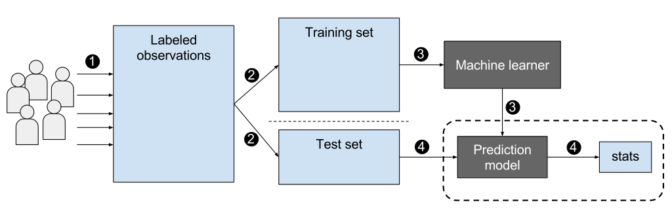
\includegraphics[width=\linewidth]{figuras/nvidia-supervised-learning.png}
    \caption{Aprendizado supervisionado \hl{OBS: COLOCAR FONTE}}
    \label{fig:nvidia-supervised-learning}
  \end{figure}
  \newpage
  \item \textbf{Aprendizado não supervisionado:} diz respeito aos métodos de aprendizagem de máquina os quais utiliza-se como dado de entrada um dado que não possui nenhum tipo de anotação e que, muitas vezes, sua estrutura é desconhecida.

  Tal processo de aprendizagem permite extrair características relevantes sobre o dado que possam servir de insumo para uma futura categorização e classificação do mesmo. Dependendo do problema em questão, a aprendizagem supervisionada pode organizar o dado em diferentes categorias \cite{learning-types} como clusterização, associação, \textit{autoencoders}, \textit{anomaly detection}, etc.

  \item \textbf{Aprendizado semi-supervisionado:} já o aprendizado semi-supervisionado junta um pouco dos dois mundos: dados com registros anotados e também dados com registros não anotados. A aplicabilidade para esse tipo de aprendizagem é quando se possui um dado onde não é trivial extrair informações relevantes sobre ele e tampouco é realizar toda a anotação da amostra em questão \cite{learning-types}.
\end{itemize}

Dentro dos tipos de algoritmos que podem ser utilizados para construir ML, um que é bastante notado, se não o mais conhecido, são as chamadas Redes Neurais Artificiais ou \textit{Neural Networks} (NN). Diferentemente de \textit{Machine Learning}, as NN é um campo dentro de ML que possiblita o aprendizado de máquina tentando imitar o comportamento dos neurônios humanos \cite{neural-net-history}.

\subsection{\textit{Neural Networks}}

Em 1943, Warren McCullock e Walter Pitts em seu artigo \textit{A Logical Calculus of the Ideas Immanent in Nervous Activity} desenvolveram um estudo para tentar explicar como o cérebro consegue reconhecer um nível complexo de padrões por meio dos neurônios \cite{first-neuron-study}, desenvolvendo um modelo chamado MCP (McCullock-Pitts), que atualmente é conhecido como o ancestral das redes neurais artificiais \cite{dl-brief-review}. Tal estudo possibilitou dar-se o pontapé para a evolução das redes neurais que conhecemos hoje.

Na década de 1950 surgiu então o modelo de \textit{Perceptron} \cite{perceptron}, que é a primeira rede neural formalmente desenvolvida composta de apenas uma única camada, descrito como um modelo matemático que recebe várias entradas e produz uma saída binária.

% fonte da imagem: https://towardsdatascience.com/the-perceptron-3af34c84838c

\begin{figure}[h]
  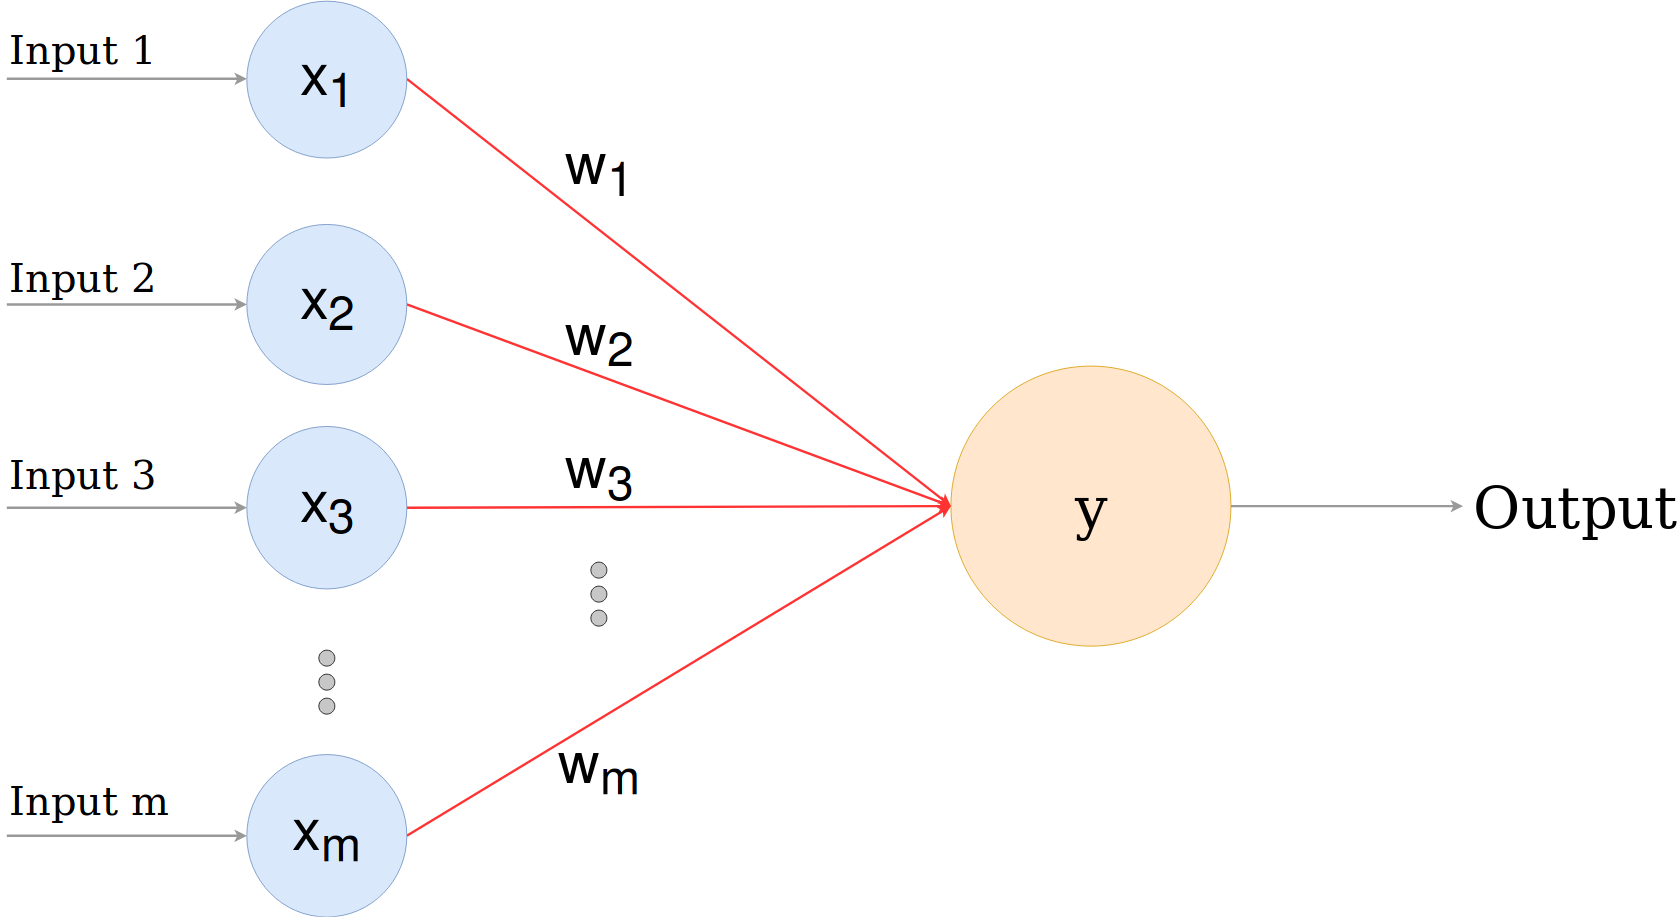
\includegraphics[width=13cm, center]{figuras/perceptron}
  \caption{O \textit{Perceptron} \hl{OBS: COLOCAR FONTE}}
  \label{fig:perceptron}
\end{figure}

Cada entrada ou \textit{input} representa um dado de entrada que são inseridos diretamente nos nós de entrada ou \textit{input nodes}, representados pela letra \(x\). Cada um desses nós representam separadamente uma característica do dado de entrada. Na figura \ref{fig:perceptron}, a quantidade de características é delimitada pela letra \(m\) e o intervalo de características é dado por [1, \(m\)]. A camada caracterizada pelas letras \textit{x} é chamada de camada de entrada ou \textit{input layer}. Redes Neurais só podem receber como entrada valores numéricos \cite{deep-learning-book}.

É importante reparar na figura \ref{fig:perceptron} que todo nó da camada de entrada está diretamente associado com uma seta caracterizada pela letra \(w\), também de intervalo [1, \(m\)]. Tais letras caracterizam o que é conhecido como os pesos ou \textit{weights}. As setas são chamadas de sinapses\footnote
{
  Na biologia, sinapse é a região localizada entre os neurônios e agem como neurotransmissores, responsáveis por realizar a transferência de inpulso nervoso de um neurônio para o outro \cite{synapses}.
}.
Essa região é definida como camada de pesos ou \textit{weight layer}.

Por fim, tem-se o nó de maior tamanho definido pela letra \(y\), conhecido como nó de saída ou \textit{output node}. Esse nó realiza um cálculo baseado em \textit{score} sobre os valores de entrada e peso e por meio de uma função de ativação, gera uma predição \textit{output} de 0 ou 1 sobre o valor resultante do \textit{score}.

A função matemática que define o valor encontrado em \(y\) é:

\[ y = f(x) = \sum_{i=1}^{m} x_iw_i + B\]

onde a função de ativação consome o valor resultante da função \(f(x)\), que serão melhor detalhadas na seção \ref{sssec:activation-func}. \(B\) na função define o \textit{bias} ou erro, adicionado ao valor resultante da soma de multiplicações para possíveis correções. O termo \textit{bias} foi introduzido por Tom M. Mitchell em seu artigo \textit{The Need for Biases in Learning Generalizations} \cite{biases} e o objetivo dele é possibilitar que o modelo generalize melhor o problema e seja menos sensível ao dado de entrada.

\subsubsection{Função de Ativação} \label{sssec:activation-func}

Funções de ativação são funções matemáticas que determinam o resultado de uma saída \textbf{\(z\)} de um neurônio em uma rede neural, baseando-se em um \textit{threshold}\footnote{
  o que é threshold
} \textbf{\(t\)} \hl{COLOCAR DEFINICAO}.
A partir do valor resultante \textbf{\(y\)} da soma dos valores de entrada \(x_i\) multiplicados pelos pesos \(w_i\) dentro do intervalo \([1, m]\) definido na fórmula \ref{math:weighted-sum}, se esse valor alcança ou ultrapassa o \textit{threshold}, o neurônio é ativado. Caso não alcante, ele não é ativado e seu sinal não é propagado \cite{python-ml}.

\[
  z =
  \begin{cases}
    1, & \text{se } y\geq \textit{t} \\
    0, & \text{se } y < \textit{t}
  \end{cases}
\]

A função principal das funções de ativação dentro de uma rede neural é adicionar a não-linearidade ao problema, permitindo assim que tais redes consigam computar problemas não triviais \cite{gentle-intro-to-nn}. Os principais problemas que envolvem ML, principalmente no âmbito da computação visual - foco do presente trabalho -, a porcentagem de problemas que a solução é resolvida por meio de uma equação linear é praticamente - se não - zero.

Existem diversos tipos de funções de ativação com aplicabilidade em diversos tipos de problemáticas a serem resolvidas. A figura \ref{fig:activation-functions} lista as principais e mais conhecidas funções de ativação, sendo que pesquisadores ainda realizam estudos para encontrar funções que apresentem melhores resultados \cite{intro-to-act-func}.

% fonte: https://medium.com/@shrutijadon10104776/survey-on-activation-functions-for-deep-learning-9689331ba092

\begin{figure}[H]
  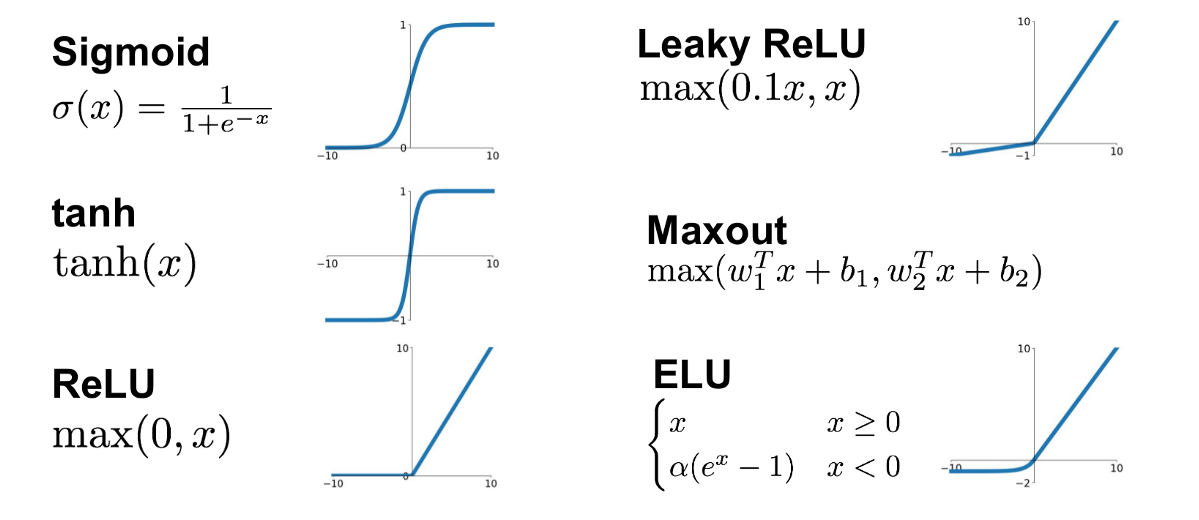
\includegraphics[width=12cm, center]{figuras/activation-functions}
  \caption{Principais funções de atiação \hl{OBS: COLOCAR FONTE}}
  \label{fig:activation-functions}
\end{figure}

\subsubsection{\textit{Weights}}

Os pesos representam o grau de conexão entre dois neurônios distintos. Por exemplo: se o peso de um neurônio 1 para o neurônio 2 tem uma maior magnitude, significa que o neurônio 1 tem maior importância sobre o neurônio 2.

Em termos práticos, o peso consegue definir o quão relevante para o problema aquele determinado valor de entrada é. Pesos que se aproximam de zero tendem a diminuir a importância do valor de entrada para o valor resultante da rede \cite{everything-about-nn}.

\subsubsection{\textit{Forward pass}}

\subsubsection{\textit{Backpropagation}}

\subsubsection{Hiperparâmetros}

\subsubsection{CNN}

\subsection{Discriminativo vs Generativo}

\section{OCR}